<%! import os, re %>

<%def name="image(path, file, caption='', label='')">

    <%
        image_path = os.path.join(path, file)
        
        if not os.path.isabs(image_path):
            image_label, ext = os.path.splitext(image_path)
            image_path = os.path.join(base_path, image_path)
        else:
            image_label, ext = os.path.splitext(file)
        
        image_path = image_path.replace('\\','/')
        if not os.path.exists(image_path):
            image_path = '../image.jpg'
            
	if len(label)>0:
	    image_label = label
	else:
            image_label = image_label.replace('/','_').replace('\\','_')
            image_label = re.sub('_+', '_', image_label)

    %>
    
    \begin{figure}[H]
        \centering
        \includegraphics[width=100mm]{${image_path}}
        \caption{${caption}}
        \label{fig:${image_label}}
    \end{figure}

</%def>

<%def name="table(path, file, caption='', label='')">

    \begin{table}[H]
        \centering
            
        <%
            table_path = os.path.join(path, file)
            
            if not os.path.isabs(table_path):
                table_label, ext = os.path.splitext(table_path)
                table_path = os.path.join(base_path, table_path)
	    else:
	        table_label, ext = os.path.splitext(file)
	    
	    tabular = ''
	    if os.path.exists(table_path):
                f = open(table_path, 'r')
                tabular = f.read()
                f.close()
                
            if len(label)>0:
                table_label = label
            else:
                table_label = table_label.replace('/','_').replace('\\','_')
                table_label = re.sub('_+', '_', table_label)
        %>
    
        % if tabular:
        
        ${tabular}	
        
        % else:
        
        \caption{${caption}}
        \begin{tabular}{c}
            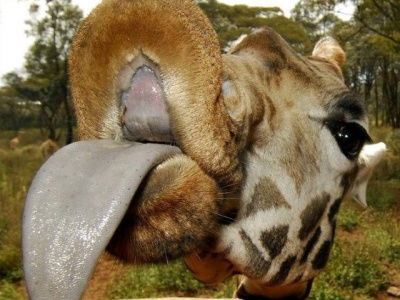
\includegraphics[width=50mm]{../table.jpg} \\
        \end{tabular}
        
        % endif
        
        \label{tab:${table_label}}
    \end{table}
    
</%def>

<%def name="latex_escape(string)">

<%
    replacements = ('&', '\\$', '%', '_', '#', '\\{', '\\}');
    
    for s in replacements:
        string = re.sub(r'([^\\]?)'+s, r'\1\\'+s, string)
        
    replacements = {'^':'\\^{}', '~':'\\~{}', '|':'\\textbar ', '<':'\\textless ', '>':'\\textgreater '};
        
    for s, r in replacements.iteritems():
        string = string.replace(s, r)
            
    return string
%>
    
</%def>